\documentclass[12pt]{article}
\author{Mengxiao}
	\title{Cpts570-hw3}
	\usepackage{graphicx}
\begin{document}
	\maketitle
	\pagebreak
	\section{Analytical Part}
		\subsection{Problem 1}
			\subsubsection{a.}
				According to the Jensen's inequality,
				$$f(E[X])\leq E[f(X)]$$
				Let $f(y)=y^2$, and we can get:
				$$f(E[X])=f(E[x_i-y_i])=(\frac{1}{d}\sum_{i=1}^d(x_i-z_i))^2=\frac{1}{d}(\frac{1}{\sqrt{d}}\sum_{i=1}^d(x_i-z_i))^2$$
				$$E[f(X)]=\frac{1}{d}\sum_{i=1}^d(x_i-z_i)^2$$
				Then, according to $f(E[X])\leq E[f(X)]$:
				$$(\frac{1}{\sqrt{d}}\sum_{i=1}^dx_i-\frac{1}{\sqrt{d}}\sum_{i=1}^dz_i)^2\leq\sum_{i=1}^d(x_i-z_i)^2$$
			\subsubsection{b.}
				According to the above property, we can know that $\sqrt{(\frac{1}{\sqrt{d}}\sum_{i=1}^dx_i-\frac{1}{\sqrt{d}}\sum_{i=1}^dz_i)^2}$ is less than the distance, so that we can use this to approximate the disatance. And it can be simpled to $|\sum_{i=1}^d(x_i-z_i)|$
		\subsection{Problem 2}
			In the article, the author mainly talk about two things:1. Some nearest neighbor algorithms based on locality-sensitive hashing(LSH). 2. a new algorithm that based on hashing and used for points in d-dimensional Euclidean space has a good optimal during LSH algorithm. If the number of dimensions is very large, there is little improvement over a linear time algorithm that compares a query to each point from the database, called “the curse of dimensionality.” The LSH algorithm can be used to reduce the dimensionality for the near neighbor search. A LSH family $H$ is called $(R,cR,P_1,P_2)-sensitive$ if for any two points$p,q\in R^d$:
\\if $||p-q||\leq R$ then $Pr_H[h(q)=h(p)]\geq P_1$,
\\if $||p-q||\geq cR$ then $Pr_H[h(q)=h(p)]\leq P_2$.
\\It is useful when $P_1>P_2$.\\
			In this article, the author yield a new LSH family that $\rho(c)=\frac{1}{c^2}$+O(loglog$n$/log$^\frac{1}{3}n)$. For infinity $w$, it will tends to $\frac{1}{c}$. For small values of $w$, it will lies slightly below $\frac{1}{c}$.
		\subsection{Problem 3}
			I think we can build such equivalent decision tree, if the set of rules contains completion if-then rules. Since, if we only have "if a$>$10, then" and don't have "if a$\leq$10, then", we can only build a part of a decision tree.
		\subsection{Problem 4}
			When we do generative classifiers, we will use joint probability $p(x,y)$ to calculate $p(y|x)$ with Bayes ruls. When we do discriminative classifiers, we will directly calculate $p(y|x)$. The bayes classifier and logistical regression will form a Generative-Discriminative pair andthe asymptotic sample complexity is $O(\log{n})$. \\
	Also, the logistical regression will seldom has lower performance, if there are not small datasets that will let logistical regression hasn't expected dominance. At most of the time, the asymptotic error of discriminative logistical classification will lower than Bayes classification, but the Bayes classifier will have a higher speed of converge.
		\subsection{Problem 5}
			\subsubsection{a.}
				Since the training data approaches infinity, the logistic regression will have a better performance. The Logistic Regression is a discriminative classifier and Naive Bayes is a generative classifier, according to the paper above, discriminative logistical regression will have a lower asymptotic error.
			\subsubsection{b.}
				If the training data doesn't satisfy the Naive Bayes assumption, the Logistic Regression will still have a higher performance than Naive Bayes, the reason is as before.
			\subsubsection{c.}
				Yes we can. Since Naive Bayes classifier is based on all the $P$.
			\subsubsection{d.}
				No, we directly get $P(Y|X)$ from the data by logistic regression. 
		\subsection{Problem 6}
				The main topic of machine learning is supervised learning that we are focusing on labeled data. Overfitting is that we try too much work on the training data that it is fit the training data on it's typical model like noisy instead of the real situation. We can try to use the sub-optimal algorithms instead of global optimal algorithms to keep away from overfitting.
		\subsection{Problem 7}
			The main topic of this paper is that statistical methods nowadays cannot solve the problem and a new method has been mentioned in this paper. It's really important to make the method be diversity since it can avoid the classification make similar errors on some data. There are three reasons for constructing ensembles. 1. Construct an ensemble can let the number of votes decrease in the classification, it will also decrease the probability of mistakes in statistics. 2. The local optimal search may have better performance on approximation than global optimal algorithms, the global optimal algorithm will have some problem during computing. 3. The last reason is that expand the space of representable function is possible when using weighted sums of hypotheses. We can use a lot of methods like Bayesian Voting to build ensembles.
 	\section{Programming and Empirical Analysis Part}
		\subsection {Naive Bayes}
			I have get 60\% of the accuracy at training data and close to 80\% at testing data.
		\subsection {CNN}
            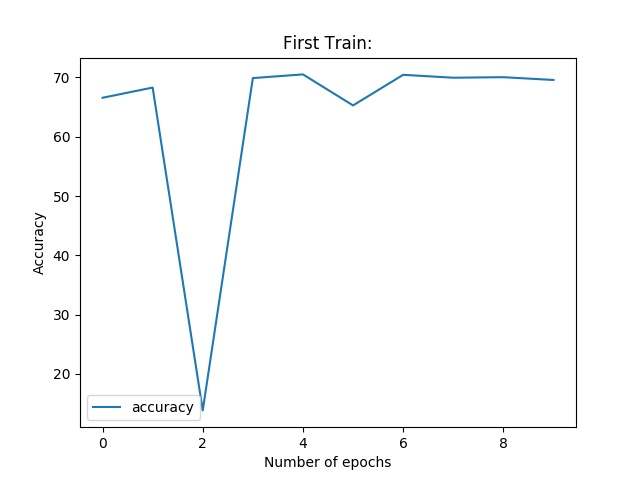
\includegraphics[height=10cm]{hw3_b_1}\\
            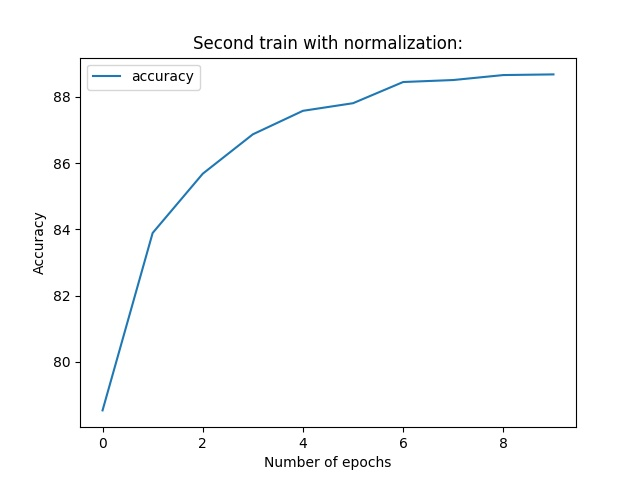
\includegraphics[height=10cm]{hw3_b_2}\\
			The accuracy at first can be 70\%. Then I try to do the normalization, then it will attach at most 90\%. Normalization is so important.
\end{document}
